%\documentclass[12pt]{article}

\questionheader{ex:s4.1}

%%%%%%%%%%%%%%%%%%
\subsection*{\Conceptual}
%%%%%%%%%%%%%%%%%%

%%%%%%%%%%%%%%%%%%%%%%%%%%%%%%%
\begin{question}[M317 2012J] %2
Let $\vF = P\,\hi + Q\,\hj$ be the two dimensional vector field
shown below.


\begin{enumerate}[(a)]
\item
Assuming that the vector field in the picture is a force field, the work 
done by the vector field on a particle moving from point $A$ to $B$ 
along the given path is:
\begin{enumerate}[(A)]
\item  Positive
\item  Negative
\item  Zero
\item Not enough information to determine.
\end{enumerate}

\item
Which statement is the most true about the line integral
$\int_{C_2} \vF\cdot\dee{\vr}$:
\begin{enumerate}[(A)]
\item  $\int_{C_2} \vF\cdot\dee{\vr}>0$
\item  $\int_{C_2} \vF\cdot\dee{\vr}=0$
\item  $\int_{C_2} \vF\cdot\dee{\vr}<0$
\item Not enough information to determine.
\end{enumerate}

\goodbreak

\begin{center}
    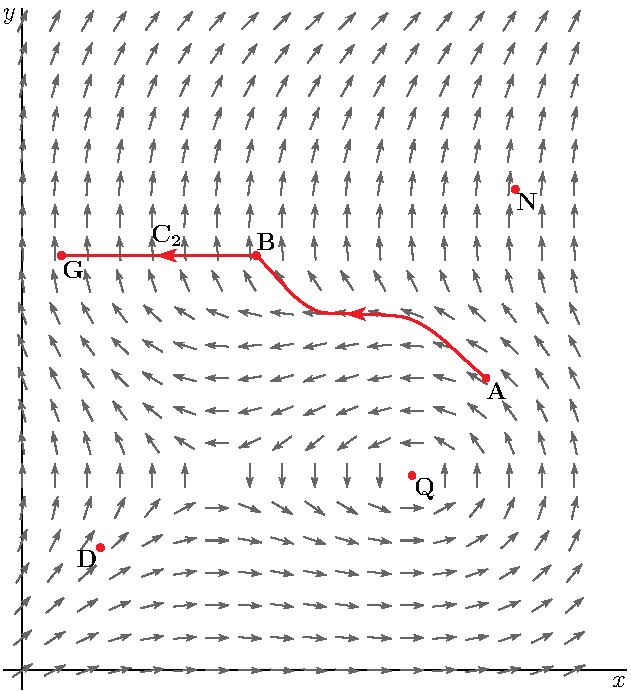
\includegraphics{OE12J_2.pdf}
\end{center}

\item 
$\vnabla\cdot\vF$ at the point $N$ (in the picture) is:
\begin{enumerate}[(A)]
\item Positive
\item Negative
\item Zero
\item Not enough information to determine.
\end{enumerate}

\item 
$Q_x - P_y$ at the point $Q$ is:
\begin{enumerate}[(A)]
\item Positive
\item Negative
\item Zero
\item Not enough information to determine.
\end{enumerate}


\item 
Assuming that $\vF = P\,\hi + Q\,\hj$, which of the following 
statements is correct about $\frac{\partial P}{\partial x}$ 
at the point $D$?
\begin{enumerate}[(A)]
\item $\frac{\partial P}{\partial x}=0$  at $D$.
\item $\frac{\partial P}{\partial x}>0$  at $D$.
\item $\frac{\partial P}{\partial x}<0$  at $D$.
\item The sign of $\frac{\partial P}{\partial x}$ 
at $D$ can not be determined by the given information.
\end{enumerate}

\end{enumerate}



\end{question}

%\begin{hint} 
%
%\end{hint}

\begin{answer}
(a) A\qquad
(b) B\qquad
(c) C\qquad
(d) A\qquad
(e) B 
\end{answer}

\begin{solution} 
(a)
A. The angle between $\vF$ and $\dee{\vr}$ is less than $90^\circ$
along the entire path. So $\vF\cdot\dee{\vr}>0$ along the entire path and
the work is positive.

(b) 
B. $\vF$ is perpendicular to $\dee{\vr}$ along all of $C_2$.
So $\int_{C_2} \vF\cdot\dee{\vr}=0$.

(c)
C. It looks like $P_x=Q_y=0$ at $N$. So $\vnabla\cdot\vF=0$ at $N$.

(d) 
A. At $Q$, the vertical component of $\vF$ is increasing from left to right
(so that $Q_x>0$) and the horizontal component of $\vF$  is decreasing
from bottom to top (so that $P_y<0$). So $Q_x - P_y>0$ at $N$.

(e) 
B. At $D$,  the horizontal component of $\vF$  is increasing
from left to right, so that $P_x>0$.
\end{solution}

%%%%%%%%%%%%%%%%%%%%%%%%%%%
\begin{question}
Does $\vnabla\times \vF$ have to be perpendicular to $\vF$?
\end{question}

\begin{hint} 
Compute $\vnabla\times \vF$ for some simple vector fields.
\end{hint}

\begin{answer} 
No.
\end{answer}

\begin{solution} 
No.  The vector field $\vF(x,y,z) = \hi +y\,\hk$ has
\begin{align*}
\vnabla\times \vF
&=\det\left[\begin{matrix} \hi & \hj & \hk \\
                           \pdiff{}{x} & \pdiff{}{y} & \pdiff{}{z} \\
                           1 & 0 & y
            \end{matrix}\right] \\
&=\hi
\end{align*}
has dot product $1$ with $\vF(x,y,z)$ (for all $x$, $y$, $z$) and
so is not perpendicular to it.
\end{solution}

%%%%%%%%%%%%%%%%%%%%%%%%%%%%
\begin{question}
Verify the vector identities
\begin{enumerate}[(a)]
\item
$\vnabla\cdot(f\vF)=f\vnabla\cdot\vF+\vF\cdot\vnabla f$
\item
$\vnabla\cdot(\vF\times\vG)
                      =\vG\cdot(\vnabla\times\vF)-
                       \vF\cdot(\vnabla\times\vG)$
\item
$\vnabla^2(fg)=f\,\vnabla^2 g+2\vnabla f\cdot\vnabla g+g\,\vnabla^2 f$
\end{enumerate}

\end{question}

\begin{hint} 
For parts(a) and (b), write out the definitions of the left and right
hand sides and observe that they are equal.
Part (c) can be done easily by using other, simpler, vector identities.
\end{hint}

\begin{answer} 


\end{answer}

\begin{solution} 
(a) By the product rule
\begin{align*}
\vnabla\cdot(f\vF)
&=\pdiff{}{x}(fF_1)
 +\pdiff{}{y}(fF_2)
 +\pdiff{}{z}(fF_3) \\
&=\phantom{+}f\pdiff{F_1}{x}
 +f\pdiff{F_2}{y}
 +f\pdiff{F_3}{z} \\
&\phantom{=}+F_1\pdiff{f}{x}
 +F_2\pdiff{f}{y}
 +F_3\pdiff{f}{z} \\
&=f\,\vnabla\cdot\vF+\vF\cdot\vnabla f
\end{align*}

(b) Again by the product rule
\begin{align*}
\vnabla\cdot(\vF\times\vG)
&=\pdiff{}{x}(F_2G_3-F_3G_2)
 +\pdiff{}{y}(F_3G_1-F_1G_3)
 +\pdiff{}{z}(F_1G_2-F_2G_1) \\
&=\phantom{+}\pdiff{F_2}{x}G_3
        -\pdiff{F_3}{x}G_2
 +\pdiff{F_3}{y}G_1
        - \pdiff{F_1}{y}G_3
 +\pdiff{F_1}{z}G_2
       - \pdiff{F_2}{z}G_1 \\
&\phantom{=}+F_2\pdiff{G_3}{x}
       -F_3\pdiff{G_2}{x}
 +F_3\pdiff{G_1}{y}
       -F_1\pdiff{G_3}{y}
 +F_1\pdiff{G_2}{z} 
      - F_2\pdiff{G_1}{z} \\
&=\phantom{+}
  \left(\pdiff{F_3}{y}-\pdiff{F_2}{z}\right)G_1
  +\left(\pdiff{F_1}{z}-\pdiff{F_3}{x}\right)G_2
  +\left(\pdiff{F_2}{x}-\pdiff{F_1}{y}\right)G_3 \\
&\phantom{=}
  -F_1\left(\pdiff{G_3}{y}-\pdiff{G_2}{z}\right)
  -F_2\left(\pdiff{G_1}{z}-\pdiff{G_3}{x}\right)
  -F_3\left(\pdiff{G_2}{x}-\pdiff{G_1}{y}\right)
\\
&=\vG\cdot(\vnabla\times\vF)-
                       \vF\cdot(\vnabla\times\vG)
\end{align*}

(c) Recall that $\vnabla^2(fg) = \vnabla\cdot\big[\vnabla(fg)\big]$.
First
\begin{align*}
\vnabla(fg)
&=\hi\pdiff{}{x}(fg)
 +\hj\pdiff{}{y}(fg)
 +\hk\pdiff{}{z}(fg) \\
&=\phantom{+}\hi g\pdiff{f}{x}
 +\hj g\pdiff{f}{y}
 +\hk g\pdiff{f}{z} \\
&\phantom{=}+\hi f\frac{\partial g}{\partial x}
 +\hj f\frac{\partial g}{\partial y}
 +\hk f\frac{\partial g}{\partial z} \\
&=g\vnabla f+f\vnabla g
\end{align*}
So by part (a), twice,
\begin{align*}
\vnabla^2(fg)
& = \vnabla\cdot\big(g\vnabla f\big)
   +\vnabla\cdot\big(f\vnabla g\big) \\
&= g\big(\vnabla\cdot \vnabla f\big) 
          + \big(\vnabla g\big)\cdot\big(\vnabla f\big)
   +f\big(\vnabla\cdot\vnabla g\big)
       + \big(\vnabla f\big)\cdot\big(\vnabla g\big) \\
&=f\,\vnabla^2 g+2\vnabla f\cdot\vnabla g+g\,\vnabla^2 f
\end{align*}
\end{solution}


%%%%%%%%%%%%%%%%%%
\subsection*{\Procedural}
%%%%%%%%%%%%%%%%%%

%%%%%%%%%%%%%%%%%%%%%%%%%%%%
\begin{question}
Evaluate $\vnabla\cdot\vF$ and $\vnabla\times\vF$ for each of
the following vector fields.
\begin{enumerate}[(a)]
\item $\vF=x\,\hi+y\,\hj+z\,\hk$ 
\item $\vF=xy^2\hi-yz^2\hj+zx^2\hk$ 
\item $\vF=\frac{x\hi+y\hj}{\sqrt{x^2+y^2}}$ 
               (the polar basis vector $\hat{\bf r}$ in 2d)
\item
$\vF=\frac{-y\hi+x\hj}{\sqrt{x^2+y^2}}$ 
      (the polar basis vector $\hat{\pmb{\theta}}$ in 2d)
\end{enumerate}

\end{question}

%\begin{hint} 
%\end{hint}

\begin{answer} 
(a) $\vnabla\cdot\vF=3$, $\vnabla\times\vF=\vZero$

(b) $\vnabla\cdot\vF=y^2-z^2+x^2$, 
    $\vnabla\times\vF=2yz\,\hi-2xz\,\hj-2xy\,\hk$

(c) $\vnabla\cdot\vF=\frac{1}{\sqrt{x^2+y^2}}$, 
    $\vnabla\times\vF=\vZero$

(d) $\vnabla\cdot\vF=0$, $\vnabla\times\vF=\frac{\hk}{\sqrt{x^2+y^2}}$

\end{answer}

\begin{solution} 
(a)
By definition
\begin{align*}
\vnabla\cdot(x\,\hi+y\,\hj+z\,\hk)
&=\pdiff{}{x}\big(x\big)
  +\pdiff{}{y}\big(y\big)
  +\pdiff{}{z}\big(z\big)
=  3 \\
\vnabla\times(x\,\hi+y\,\hj+z\,\hk)
&=\det\left[\begin{matrix}\hi & \hj & \hk \\[0.05in]
                  \pdiff{}{x} &
                  \pdiff{}{y} &
                  \pdiff{}{z} \\[0.05in]
                  x & y & z\end{matrix}\right]
= \vZero
\end{align*}

(b)
By definition
\begin{align*}
\vnabla\cdot(xy^2\hi-yz^2\hj+zx^2\hk)
&=\pdiff{}{x}\big(xy^2\big)
  +\pdiff{}{y}\big(-yz^2\big)
  +\pdiff{}{z}\big(zx^2\big)
=y^2-z^2+x^2 \\
\vnabla\times(xy^2\hi-yz^2\hj+zx^2\hk)
&=\det\left[\begin{matrix}\hi & \hj & \hk \\[0.05in]
                  \pdiff{}{x} &
                  \pdiff{}{y} &
                  \pdiff{}{z} \\[0.05in]
                  xy^2 & -yz^2 & zx^2\end{matrix}\right]
= 2yz\,\hi-2xz\,\hj-2xy\,\hk
\end{align*}

(c)
By definition
\begin{align*}
\vnabla\cdot\left(\frac{x}{\sqrt{x^2+y^2}}\hi+\frac{y}{\sqrt{x^2+y^2}}\hj\right)
&=\pdiff{}{x}\left(\frac{x}{\sqrt{x^2+y^2}}\right)
  +\pdiff{}{y}\left(\frac{y}{\sqrt{x^2+y^2}}\right) \\
&= \frac{1}{\sqrt{x^2+y^2}} - \frac{x^2}{{[x^2+y^2]}^{3/2}}
   +\frac{1}{\sqrt{x^2+y^2}} - \frac{y^2}{{[x^2+y^2]}^{3/2}} \\
&=\frac{x^2+y^2\ -x^2\ +x^2+y^2\ -\ y^2}{{[x^2+y^2]}^{3/2}} \\
&=\frac{1}{\sqrt{x^2+y^2}} \\
\vnabla\times\left(\frac{x}{\sqrt{x^2+y^2}}\hi+\frac{y}{\sqrt{x^2+y^2}}\hj\right)
&=\det\left[\begin{matrix}\hi & \hj & \hk \\[0.05in]
                  \pdiff{}{x} &
                  \pdiff{}{y} &
                  \pdiff{}{z} \\[0.05in]
                  \frac{x}{\sqrt{x^2+y^2}} & 
                  \frac{y}{\sqrt{x^2+y^2}} & 0\end{matrix}\right] \\[0.05in]
&=\left(- \frac{xy}{{[x^2+y^2]}^{3/2}}+ \frac{xy}{{[x^2+y^2]}^{3/2}}\right)\hk
= \vZero
\end{align*}

(d)
By definition
\begin{align*}
\vnabla\cdot\left(-\frac{y}{\sqrt{x^2+y^2}}\hi+\frac{x}{\sqrt{x^2+y^2}}\hj\right)
&=\pdiff{}{x}\left(-\frac{y}{\sqrt{x^2+y^2}}\right)
  +\pdiff{}{y}\left(\frac{x}{\sqrt{x^2+y^2}}\right) \\
&=  \frac{xy}{{[x^2+y^2]}^{3/2}}
   - \frac{xy}{{[x^2+y^2]}^{3/2}} 
=0 \\
\vnabla\times\left(-\frac{y}{\sqrt{x^2+y^2}}\hi
                         +\frac{x}{\sqrt{x^2+y^2}}\hj\right)
&=\det\left[\begin{matrix}\hi & \hj & \hk \\[0.05in]
                  \pdiff{}{x} &
                  \pdiff{}{y} &
                  \pdiff{}{z} \\[0.05in]
                  -\frac{y}{\sqrt{x^2+y^2}} & 
                  \frac{x}{\sqrt{x^2+y^2}} & 0\end{matrix}\right] \\[0.05in]
&=\!\left(\!\frac{1}{\sqrt{x^2+y^2}} - \frac{x^2}{{[x^2+y^2]}^{3/2}}
   +\frac{1}{\sqrt{x^2+y^2}} - \frac{y^2}{{[x^2+y^2]}^{3/2}}\!\right)\!\hk
\\
&= \frac{x^2+y^2\ -x^2\ +x^2+y^2\ -\ y^2}{{[x^2+y^2]}^{3/2}}\ \hk 
= \frac{\hk}{\sqrt{x^2+y^2}}
\end{align*}
\end{solution}

%%%%%%%%%%%%%%%%%%%%%%%%%%%
\begin{question}[M317 2015A] %1 a,b
\begin{enumerate}[(a)]
\item
Compute and simplify $\vnabla\cdot\big(\frac{\vr}{r}\big)$
for $\vr=(x,y,z)$ and $r=|(x,y,z)|$. Express your answer in 
terms of $r$.

\item
Compute $\vnabla\times\big(yz\,\hi + 2xz\,\hj + e^{xy}\,\hk\big)$.
\end{enumerate}

\end{question}

%\begin{hint} 
%\end{hint}

\begin{answer} 
(a) $\frac{2}{r}$\qquad
(b) $\big(xe^{xy}-2x\big)\,\hi+y\big(1-e^{xy}\big)\,\hj+z\,\hk$
\end{answer}

\begin{solution} (a)
 We are to compute the divergence of $\frac{\vr}{r}
=\frac{x\,\hi+y\,\hj+z\,\hk}{[x^2+y^2+z^2]^{1/2}}$. Since
\begin{alignat*}{3}
\pdiff{}{x}\frac{x}{{[x^2+y^2+z^2]}^{1/2}}
&=\frac{1}{{[x^2+y^2+z^2]}^{1/2}} 
            -\frac{1}{2}\frac{x(2x)}{{[x^2+y^2+z^2]}^{3/2}}
&\,=\,\frac{y^2+z^2}{{[x^2+y^2+z^2]}^{3/2}}
\\
\pdiff{}{y}\frac{y}{{[x^2+y^2+z^2]}^{1/2}}
&=\frac{1}{{[x^2+y^2+z^2]}^{1/2}} 
            -\frac{1}{2}\frac{y(2y)}{{[x^2+y^2+z^2]}^{3/2}}
&\,=\,\frac{x^2+z^2}{{[x^2+y^2+z^2]}^{3/2}}
\\
\pdiff{}{z}\frac{z}{{[x^2+y^2+z^2]}^{1/2}}
&=\frac{1}{{[x^2+y^2+z^2]}^{1/2}} 
            -\frac{1}{2}\frac{z(2z)}{{[x^2+y^2+z^2]}^{3/2}}
&\,=\,\frac{x^2+y^2}{{[x^2+y^2+z^2]}^{3/2}}
\end{alignat*}
the specified divergence is
\begin{align*}
\vnabla\left(\frac{\vr}{r}\right) &= \frac{2x^2+2y^2+2z^2}{{[x^2+y^2+z^2]}^{3/2}}
                               =\frac{2r^2}{r^3}
                               =\frac{2}{r}
\end{align*}

(b)
\begin{align*}
\vnabla\times\big(yz\,\hi + 2xz\,\hj + e^{xy}\,\hk\big)
&=\det\left[\begin{matrix}\hi&\hj&\hk\\[0.03in] 
     \pdiff{}{x}&
        \pdiff{}{y}&
        \pdiff{}{z}\\[0.03in]
yz&2xz&e^{xy}\end{matrix}\right]
=\big(xe^{xy}-2x\big)\,\hi-\big(ye^{xy}-y\big)\,\hj+z\,\hk
\end{align*}

\end{solution}


%%%%%%%%%%%%%%%%%%%%%%%%%%%
\begin{question}[M317 2008A] %5
In the following, we use the notation 
$\vr = x\,\hi + y\,\hj + z\,\hk$, $r = |\vr|$, and $k$ is some number
$k = 0, 1, -1, 2, -2, \dots$.
\begin{enumerate}[(a)]
\item
Find the value $k$ for which
\begin{equation*}
\vnabla (r^k) = -3\frac{\vr}{r^5}
\end{equation*}
\item
Find the value $k$ for which
\begin{equation*}
\vnabla  \cdot (r^k\vr) = 5r^2 
\end{equation*}
\item
Find the value $k$ for which
\begin{equation*}
\vnabla^2 (r^k) = \frac{2}{r^4}
\end{equation*}
\end{enumerate}
\end{question}

\begin{hint} 
(c) can be done efficiently by using (a) and (b).
\end{hint}

\begin{answer} 
(a) $k=-3$\qquad
(b) $k=2$\qquad
(c) $k=-2$
\end{answer}

\begin{solution} (a)
Since $r^k=\big(x^2+y^2+z^2\big)^{k/2}$,
\begin{align*}
\pdiff{}{x} r^k 
   & = 2x\ \frac{k}{2}\big(x^2+y^2+z^2\big)^{\frac{k}{2}-1}
     = k\ (\vr\cdot\hi)\ r^{k-2} \\
\pdiff{}{y} r^k 
   & = 2y\ \frac{k}{2}\big(x^2+y^2+z^2\big)^{\frac{k}{2}-1}
     = k\ (\vr\cdot\hj)\ r^{k-2} \\
\pdiff{}{z} r^k 
   & = 2z\ \frac{k}{2}\big(x^2+y^2+z^2\big)^{\frac{k}{2}-1}
     = k\ (\vr\cdot\hk)\ r^{k-2} 
\end{align*}
We want $k=-3$.

(b) Using the computation in part (a)
\begin{align*}
\vnabla  \cdot (r^k\vr) 
&= \pdiff{}{x} (x r^k)
  + \pdiff{}{y} (y r^k)
  + \pdiff{}{z} (z r^k) \\
&= 3r^k + x \pdiff{}{x} r^k
  + y \pdiff{}{y} r^k
  + z \pdiff{}{z} r^k \\
&= 3r^k + x \big(kx\ r^{k-2}\big)
  + y \big(ky\ r^{k-2}\big)
  + z \big(kz\ r^{k-2}\big) \\
&= \big(3+k\big)r^k
\end{align*}
We want $k=2$.

(c) Recalling that 
$\vnabla^2 = \vnabla\cdot\vnabla$,
\begin{align*}
\vnabla^2 (r^k )
&=\vnabla\cdot\big(\vnabla(r^k)\big) \\
&=\vnabla\cdot(k r^{k-2}\,\vr) &\text{by part (a)} \\
&=k(3+k-2)r^{k-2} &\text{by part (b),  but with $k$ replaced by $k-2$} 
\end{align*}
We want $k=-2$.

%\begin{align*}
%\vnabla^2 (r^k) 
%&= \frac{\partial^2\hfill}{\partial x^2} r^k
%  + \frac{\partial^2\hfill}{\partial y^2} r^k
%  + \frac{\partial^2\hfill}{\partial z^2} r^k \\
%&= k\pdiff{}{x} \big(x r^{k-2}\big)
%  + k \pdiff{}{y} \big(y r^{k-2}\big)
%  + k \pdiff{}{z} \big(z r^{k-2}\big) \\
%\end{align*}


\end{solution}

%%%%%%%%%%%%%%%%%%%%%%%%%%%
\begin{question}[M317 2017A] %1
Let $\vr$ be the vector field $\vr = x\,\hi + y\,\hj + z\,\hk$ and let 
$r$ be the function $r = |\vr|$. Let $\va$ be the \emph{constant} 
vector $\va = a_1\,\hi + a_2\,\hj + a_3\,\hk$. Compute and simplify 
the following quantities.
Answers must be expressed in terms of $\va$, $\vr$, and $r$. There should 
be no $x$'s, $y$'s, or $z$'s in your answers.
\begin{enumerate}[(a)]
\item
$\vnabla\cdot\vr$

\item
$\vnabla(r^2)$

\item
$\vnabla\times(\vr\times\va)$

\item
$\vnabla\cdot\big(\vnabla(r)\big)$

\end{enumerate}
\end{question}

%\begin{hint} 
%\end{hint}

\begin{answer} 
(a) $3$\qquad
(b) $2\vr$\qquad
(c) $-2\va$\qquad
(d) $\frac{2}{r}$
\end{answer}

\begin{solution} (a)
\begin{equation*}
\vnabla\cdot\vr 
=\pdiff{x}{x} 
  +\pdiff{y}{y} 
  +\pdiff{z}{z}
=3 
\end{equation*}

(b)
\begin{equation*}
\vnabla(r^2)
=\left(\hi\pdiff{}{x} 
  +\hj\pdiff{}{y} 
  +\hk\pdiff{}{z} \right)
\big(x^2+y^2+z^2\big)
=2x\,\hi +2y\,\hj +2\,\hk
=2\vr
\end{equation*}

(c) Since
\begin{equation*}
\vr\times\va = \det\left[\begin{matrix}
                         \hi & \hj & \hk \\
                          x  &  y  & z   \\
                         a_1 & a_2 & a_3 
                         \end{matrix}\right]
              =\hi\big(a_3y-a_2z\big)
              +\hj\big(a_1z-a_3x\big)
              +\hk\big(a_2x-a_1y\big)
\end{equation*}
we have
\begin{align*}
\vnabla\times(\vr\times\va)
&= \det\left[\begin{matrix}\hi&\hj&\hk\\[0.03in] 
     \pdiff{}{x}&
        \pdiff{}{y}&
        \pdiff{}{z}\\[0.03in]
    a_3y-a_2z& a_1z-a_3x & a_2x-a_1y\end{matrix}\right] 
=-2a_1\,\hi -2a_2\,\hj -2a_3\,\hk \\
 &=-2\va
\end{align*}

(d) Since
\begin{align*}
\vnabla(r) &= \left(\hi\pdiff{}{x} 
  +\hj\pdiff{}{y} 
  +\hk\pdiff{}{z} \right) \big(x^2+y^2+z^2\big)^{1/2} \\
&=\hi\frac{x}{\big(x^2+y^2+z^2\big)^{1/2}}
  +\hj\frac{y}{\big(x^2+y^2+z^2\big)^{1/2}}
  +\hk\frac{x}{\big(x^2+y^2+z^2\big)^{1/2}}
\end{align*}
we have
\begin{align*}
\vnabla\cdot\big(\vnabla(r)\big)
&= \pdiff{}{x} \frac{x}{\big(x^2+y^2+z^2\big)^{1/2}}
   +\pdiff{}{y} \frac{y}{\big(x^2+y^2+z^2\big)^{1/2}}
   +\pdiff{}{z} \frac{z}{\big(x^2+y^2+z^2\big)^{1/2}} \\
&=  \frac{3}{\big(x^2+y^2+z^2\big)^{1/2}}
   -\frac{1}{2}\frac{2x^2+2y^2+2z^2}{\big(x^2+y^2+z^2\big)^{3/2}}
 =\frac{2}{\big(x^2+y^2+z^2\big)^{1/2}} 
 =\frac{2}{r}
\end{align*} 
\end{solution}

%%%%%%%%%%%%%%%%%%%%%%%%%%%
\begin{question}[M317 2017D] %1
Let 
\begin{equation*}
\vr = x\,\hi + y\,\hj + z\,\hk,\qquad
r = |\vr|
\end{equation*}
\begin{enumerate}[(a)]
\item
Compute $a$ where $\vnabla\big(\frac{1}{r}\big) =- r^a\,\vr$.
\item
Compute $a$ where $\vnabla\cdot\big(r\,\vr\big) = ar$.
\item
Compute $a$ where $\vnabla\cdot\big(\vnabla(r^3)\big) = ar$.
\end{enumerate}
\end{question}

%\begin{hint} 
%\end{hint}

\begin{answer} 
(a) $a=-3$\qquad
(b) $a=4$\qquad
(c) $a=12$
\end{answer}

\begin{solution} (a)
Since
\begin{align*}
\vnabla\left(\frac{1}{r}\right) 
&= \left(\hi\pdiff{}{x} 
  +\hj\pdiff{}{y} 
  +\hk\pdiff{}{z} \right) \big(x^2+y^2+z^2\big)^{-1/2} \\
&=-\hi\frac{x}{\big(x^2+y^2+z^2\big)^{3/2}}
  -\hj\frac{y}{\big(x^2+y^2+z^2\big)^{3/2}}
  -\hk\frac{z}{\big(x^2+y^2+z^2\big)^{3/2}} \\
&=-\hi\frac{x}{r^3}
  -\hj\frac{y}{r^3}
  -\hk\frac{x}{r^3} 
\end{align*}
we have $a=-3$.

(b) Since
\begin{align*}
\vnabla\cdot\big(r\,\vr\big)
&= \pdiff{}{x} \Big[\big(x^2+y^2+z^2\big)^{1/2}x\Big]
   +\pdiff{}{y}\Big[\big(x^2+y^2+z^2\big)^{1/2}y\Big]
   +\pdiff{}{z} \Big[\big(x^2+y^2+z^2\big)^{1/2}z\Big] \\
&=  3\big(x^2+y^2+z^2\big)^{1/2}
   +\frac{1}{2}\frac{2x^2+2y^2+2z^2}{\big(x^2+y^2+z^2\big)^{1/2}}
 =4\big(x^2+y^2+z^2\big)^{1/2}
 =4r
\end{align*}
we have $a=4$.

(c) Since
\begin{align*}
\vnabla(r^3) &= \left(\hi\pdiff{}{x} 
  +\hj\pdiff{}{y} 
  +\hk\pdiff{}{z} \right) \big(x^2+y^2+z^2\big)^{3/2} \\
&=\hi\,3x\big(x^2+y^2+z^2\big)^{1/2}
  +\hj\,3y\big(x^2+y^2+z^2\big)^{1/2}
  +\hk\,3z\big(x^2+y^2+z^2\big)^{1/2} \\
&=3r\vr
\end{align*}
we have
\begin{align*}
\vnabla\cdot\big(\vnabla(r^3)\big)
&= \vnabla\cdot\big(3r\vr\big)
= 3\,\vnabla\cdot\big(r\vr\big) 
= 3\,\big(4r\big) \qquad\text{by part (b)} \\
&=  12 r
\end{align*}
so that $a=12$.
\end{solution}

%%%%%%%%%%%%%%%%%%%%%%%%%%%
\begin{question}
Find, if possible, a vector field $\vA$ that has $\hk$ 
component $A_3=0$ and that is a vector potential for 
\begin{enumerate}[(a)]
\item $\vF=(1+yz)\hi+(2y+zx)\hj+(3z^2+xy)\hk$
\item $\vG= yz\hi+zx\hj+xy\hk$
\end{enumerate}
\end{question}

%\begin{hint} 
%\end{hint}

\begin{answer} 
(a) $\vF$ cannot have a vector potential.

(b) Two solutions are
$\vA=\frac{1}{2}(z^2-y^2)x\hi-\frac{1}{2} yz^2\hj$ and 
$\vA=\frac{1}{2} xz^2\hi+\frac{1}{2}(x^2-z^2)y\hj$.

\end{answer}

\begin{solution} 
(a) Since 
$\vnabla\cdot\vF
=\pdiff{}{x}(1+yz)+\pdiff{}{y}(2y+zx)+\pdiff{}{z}(3z^2+xy)=2+6z\ne 0$, 
$\vF$ fails the screening test and cannot have a vector potential.

(b) The vector field $\vA=A_1\hi+A_2\hj$ is a vector
potential for $\vG$ if and only if $\vG=\vnabla\times\vA$,
which is the case if and only if
\begin{alignat*}{3}
-\pdiff{A_2}{z}&= yz\quad &
      \iff&\quad&     
      &A_2=-\frac{1}{2} yz^2+B_2(x,y)\\
\pdiff{A_1}{z}&=zx &
       \iff&\quad &  
      &A_1=\phantom{-}\frac{1}{2} xz^2+B_1(x,y)\\
\pdiff{A_2}{x}-\pdiff{A_1}{y} &=xy &
     \iff& &  & 
   \pdiff{B_2}{x} -\pdiff{B_1}{y}=xy
\end{alignat*}
There are infinitely many solutions to $\pdiff{B_2}{x}
-\pdiff{B_1}{y}=xy$. In fact $B_2$ is completely arbitrary.
If one chooses $B_2=0$, then $B_1=-\frac{1}{2} xy^2$ does the job. If one chooses
$B_1=0$, then $B_2=\frac{1}{2} x^2y$ does the job. Thus two solutions are
$\vA=\frac{1}{2}(z^2-y^2)x\hi-\frac{1}{2} yz^2\hj$ and 
$\vA=\frac{1}{2} xz^2\hi+\frac{1}{2}(x^2-z^2)y\hj$.
\end{solution}




%%%%%%%%%%%%%%%%%%
\subsection*{\Application}
%%%%%%%%%%%%%%%%%%

%%%%%%%%%%%%%%%%%%%%%%%%%%%%
\begin{question}[M317 2006D] %8
Let
\begin{align*}
\vF = \frac{-z}{x^2+z^2}\,\hi +y\,\hj +\frac{x}{x^2+z^2}\,\hk
\end{align*}

\begin{enumerate}[(a)]
\item
Determine the domain of $\vF$.
\item
Determine the curl of $\vF$. Simplify if possible.
\item
Determine the divergence of $\vF$. Simplify if possible.
\item
Is $\vF$ conservative? Give a reason for your answer.
\end{enumerate}
\end{question}

%\begin{hint} 
%
%\end{hint}

\begin{answer} 
(a) $D=\Set{(x,y,z)}{x^2+z^2\ne 0}$\qquad
(b) $\vnabla\times\vF=\vZero$ on $D$\qquad
(c) $\vnabla\cdot\vF=1$ on $D$

(d) $\vF$ is not conservative on the domain $D$ of part (a).

\end{answer}

\begin{solution}(a) $\vF$ is well-defined wherever the denominator
$x^2+z^2$ is nonzero. So the (largest possible) domain is
\begin{align*}
D=\Set{(x,y,z)}{x^2+z^2\ne 0}
\end{align*}

\noindent (b) 
As preliminary computations, let's find
\begin{align*}
\pdiff{}{z}\left(\frac{-z}{x^2+z^2}\right)
&=\frac{-1}{x^2+z^2}-\frac{2z(-z)}{{(x^2+z^2)}^2}
=\frac{-x^2+z^2}{{(x^2+z^2)}^2}
\\
\pdiff{}{x}\left(\frac{x}{x^2+z^2}\right)
&=\frac{1}{x^2+z^2}-\frac{2x(x)}{{(x^2+z^2)}^2}
=\frac{-x^2+z^2}{{(x^2+y^2)}^2}
\end{align*}
So the curl of $\vF$ is
\begin{align*}
\vnabla\times\vF
&=\det\left[\begin{matrix}
\hi &\hj &\hk \\
\tfrac{\partial\hfill}{\partial x} & \tfrac{\partial\hfill}{\partial y} & 
                \tfrac{\partial\hfill}{\partial z} \\
\frac{-z}{x^2+z^2} & y & \frac{x}{x^2+z^2}
\end{matrix}
\right]
=-\left(\frac{-x^2+z^2}{{(x^2+y^2)}^2}
  -\frac{-x^2+z^2}{{(x^2+y^2)}^2}\right)\hj
=\vZero
\end{align*}
\emph{on the domain of $\vF$}.

\noindent (c)
As preliminary computations, let's find
\begin{align*}
\pdiff{}{x}\left(\frac{-z}{x^2+z^2}\right)
&=-\frac{2x(-z)}{{(x^2+z^2)}^2}
=\frac{2xz}{{(x^2+z^2)}^2}
\\
\pdiff{}{z}\left(\frac{x}{x^2+z^2}\right)
&=-\frac{2z(x)}{{(x^2+z^2)}^2}
=\frac{-2xz}{{(x^2+y^2)}^2}
\end{align*}
So the divergence of $\vF$ is
\begin{align*}
\vnabla\cdot\vF
&=\pdiff{}{x}\left(\frac{-z}{x^2+z^2}\right)
  +\pdiff{}{y}\left(y\right)
  + \pdiff{}{z}\left(\frac{x}{x^2+z^2}\right)
=1
\end{align*}

\noindent (d) 
By part (b), the vector field passes the conservative field screening test
$\vnabla\times\vF=\vZero$. But we should still be suspicious because
of the similarity of $\vF$ to the vector field of 
Examples \eref{CLP317}{eg:screeningCounterexample} and \eref{CLP317}{eg:greenCC}
in the CLP-4 text.

So let's compute the line integral of $\vF$ around the (closed) circle
$y=0$, $x^2+z^2=1$, parametrized by
\begin{equation*}
\vr(t) = \cos t\,\hi +\sin t\,\hk\qquad
\vr'(t) = -\sin t\,\hi +\cos t\,\hk 
\end{equation*}
The line integral is
\begin{align*}
\int_C \vF \cdot \dee{\vr}
&=\int_0^{2\pi}\!\!\big\{
       \overbrace{-\sin t}^{\frac{-z}{x^2+z^2}}\,\hi
      +\overbrace{\cos t}^{\frac{x}{x^2+y^2}}\,\hk\big\}
           \cdot
  \big\{\overbrace{-\sin t\,\hi +\cos t\,\hk}^{\vr'(t)}\big\}\dee{t} \\
&= \int_0^{2\pi}\dee{t}
=2\pi
\end{align*}
As the integral of $\vF$ around the simple closed curve $C$
is not zero, $\vF$ cannot be conservative on $D$.
See Theorem \eref{CLP317}{thm:pathIndepConserv} and
Examples \eref{CLP317}{eg:screeningCounterexample} and \eref{CLP317}{eg:greenCC}
in the CLP-4 text. 

\end{solution}

%%%%%%%%%%%%%%%%%%%%%%%%%%%
\begin{question}[M317 2004A] %3
A physicist studies a vector field $\vF$ in her lab. She
knows from theoretical considerations that $\vF$ must be of the form 
$\vF=\nabla\times\vG$, for some smooth vector field $\vG$. Experiments 
also show that $\vF$ must be of the form 
\begin{equation*}
\vF(x,y,z)=(xz+xy)\hi+\alpha(yz-xy)\hj+\beta(yz+xz)\hk
\end{equation*}
where $\alpha$ and $\beta$ are constant.
\begin{enumerate}[(a)]
\item
Determine $\alpha$ and $\beta$.

\item
Further experiments show that $\vG=xyz\hi-xyz\hj+g(x,y,z)\hk$.
Find the unknown function $g(x,y,z)$.
\end{enumerate}

\end{question}

%\begin{hint} 
%\end{hint}

\begin{answer} 
(a) $\alpha=\beta=-1$

(b)  Any function of the form $g(x,y,z)=xyz+w(z)$ will work.
\end{answer}

\begin{solution} 
(a)
By the vector identity of Theorem \eref{CLP317}{thm:degTwoIdentities}.a
in the CLP-4 text,
\begin{equation*}
\nabla\cdot \vF=\nabla\cdot \nabla\times\vG=0
\end{equation*}
So we must have
\begin{equation*}
0=\nabla\cdot\vF=\nabla\cdot \big((xz+xy)\hi+\alpha(yz-xy)\hj+\beta(yz+xz)\hk\big)
=(z+y)+\alpha(z-x)+\beta(y+x)
\end{equation*}
This is true for all $(x,y,z)$ if and only if $\alpha=\beta=-1$.

(b) Since
\begin{equation*}
\nabla\times\vG=\nabla\times\big(xyz\hi-xyz\hj+g(x,y,z)\hk\big)
=(g_y+xy)\,\hi-(g_x-xy)\,hj+(-yz-xz)\,\hk
\end{equation*}
we will have that $\nabla\times\vG=\vF$ if and only if
\begin{equation*}
(g_y+xy)\,\hi-(g_x-xy)\,\hj+(-yz-xz)\,\hk=(xz+xy)\,\hi-(yz-xy)\,\hj-(yz+xz)\,\hk
\end{equation*}
which is the case if and only if
\begin{equation*}
g_y=xz,\quad g_x=yz
\end{equation*}
The first equation, $g_y=xz$, is satisfied if and only if $g=xyz+h(x,z)$.
The second equation is also satisfied if and only if
$g_x=yz+h_x(x,z)=yz$. This is the case if and only if $h_x(x,z)=0$. That
is, if and only if $h$ is independent of $x$. Equivalently, if and only
if $h(x,z)=w(z)$ for some function $w(z)$. So, in fact, any function of
the form $g(x,y,z)=xyz+w(z)$ will work.

\end{solution}


%%%%%%%%%%%%%%%%%%%%%%%%%%%
\begin{question}
A rigid body rotates at an angular velocity of $\Om$ rad/sec
about an axis that passes through the origin and has direction $\Ha$. When
you are standing at the head of $\Ha$ looking towards the origin, the rotation
is counterclockwise. Set $\vOm=\Om\Ha$. 
\begin{enumerate}[(a)]  
\item
Show that the velocity of the point $\vr=(x,y,z)$ on the body is $\vOm\times\vr$.
\item
Evaluate $\vnabla\times(\vOm\times\vr)$ and  
$\vnabla\cdot(\vOm\times\vr)$, treating $\vOm$ as a constant.
\item
Find the speed of the students in a classroom located at
latitude $49^\circ$ N due to the rotation of the Earth. Ignore the motion
of the Earth about the Sun, the Sun in the Galaxy and so on. The radius
of the Earth is 6378 km.
\end{enumerate}
\end{question}

\begin{hint} 
(a) Find the magnitude and direction of the velocity vector.
Then verify that $\vOm\times\vr$ has that magnitude and direction.
\end{hint}

\begin{answer} 
(a) See the solution

(b) $\vnabla\times(\vOm\times\vr)=2\vOm\qquad \vnabla\cdot(\vOm\times\vr)=0$
\qquad
(c) $1095$km/hr

\end{answer}

\begin{solution} 
(a)
 Denote by $\theta$ the angle between $\Ha$ and $\vr$.
The point $\vr$ is a distance $\ell=|\vr|\,\sin\theta$ from the axis
of rotation. So as the body rotates, the point sweeps out a circle of radius
$\ell$ centred on the axis of rotation.
\vadjust{
\begin{center}
    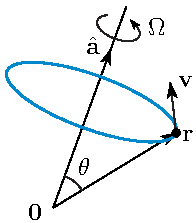
\includegraphics{rigid.pdf}
\end{center}
}%
In one second the point sweeps
out an arc of this circle that subtends an angle of $\Om$ radians. This arc
is the fraction $\frac{\Om}{2\pi}$ of a full circle and so has length
$\frac{\Om}{2\pi}2\pi \ell=\Om\ell=\Om|\vr|\,\sin\theta$. Thus the point
is moving with speed $\Om|\vr|\,\sin\theta$. The velocity vector of the
point must have length $\Om|\vr|\,\sin\theta$ and direction perpendicular
to both $\Ha$ and $\vr$. The vector 
$\vOm\times\vr$ is perpendicular to both  $\vr$ and $\vOm=\Om\Ha$
and has length
$\ 
|\vOm|\,|\vr|\,\sin\theta
=\Om|\vr|\,\sin\theta
\ $
as desired. So the velocity vector is either
$\vOm\times\vr$ or its negative. By the right hand rule it is $\vOm\times\vr$.
\smallskip

(b) By vector identities 
\begin{align*}
\vnabla\cdot(\vF\times\vG)
   &=\vG\cdot(\vnabla\times\vF)-\vF\cdot(\vnabla\times\vG)\\
\vnabla\times(\vF\times\vG)
   &=\vF(\vnabla\cdot\vG)-(\vnabla\cdot\vF)\vG
+(\vG\cdot\vnabla)\vF-(\vF\cdot\vnabla)\vG
\end{align*} 
(which are Theorems \eref{CLP317}{thm:divIdentities}(d)  
and \eref{CLP317}{thm:curlIdentities}(d) in the CLP-4 text)
and the assumption that $\vOm$ is constant
\begin{align*}
\vnabla\times(\vOm\times\vr)&=
\vOm(\vnabla\cdot\vr)-(\vnabla\cdot\vOm)\vr
+(\vr\cdot\vnabla)\vOm-(\vOm\cdot\vnabla)\vr
=\vOm(\vnabla\cdot\vr)-(\vOm\cdot\vnabla)\vr\\
\vnabla\cdot(\vOm\times\vr)&=
\vr\cdot(\vnabla\times\vOm)-
\vOm\cdot(\vnabla\times\vr)
=-\vOm\cdot(\vnabla\times\vr)
\end{align*}
Substituting in
\begin{align*}
\vnabla\cdot\vr&=\pdiff{x}{x}+
\pdiff{y}{y}+\pdiff{z}{z}=3\\
\vnabla\times\vr
&=\big(\pdiff{z}{y}-\pdiff{y}{z}\big)\hi+
\big(\pdiff{x}{z}-\pdiff{z}{x}\big)\hj
+\big(\pdiff{y}{x}-\pdiff{x}{y}\big)\hk
=\vZero\\
(\vOm\cdot\vnabla)\vr&=
\big(\Om_1\pdiff{}{x}
+\Om_2\pdiff{}{y}
+\Om_3\pdiff{}{z}\big)
\big(x\hi+y\hj+z\hk\big)
=\Om_1\hi+\Om_2\hj+\Om_3\hk=\vOm
\end{align*}
gives
\begin{equation*}
\vnabla\times(\vOm\times\vr)=2\,\vOm\qquad \vnabla\cdot(\vOm\times\vr)=0
\end{equation*}

(c)
The students are a distance $6378\sin(90^\circ- 49^\circ)=
6378\cos(49^\circ)=4184$ km from the axis of rotation. The rate of rotation
is $\Om =\frac{2\pi}{24}$ radians per hour. In each hour the students
sweep out an arc of $\frac{2\pi}{24}$ radians from a circle of radius
$4184$ km. Their speed is $\frac{2\pi}{24}\times 4184=1095$km/hr.
\end{solution}

%%%%%%%%%%%%%%%%%%%%%%%%%%%
\begin{question}
Suppose that the vector field $\vF$ obeys $\vnabla\cdot \vF=0$ in
all of $\bbbr^3$. Let 
\begin{equation*}
\vr(t)=tx\,\hi+ty\,\hj+tz\,\hk,\qquad 0\le t\le 1
\end{equation*}
be a parametrization of the line segment from the origin to $(x,y,z)$. Define
\begin{equation*}
\vG(x,y,z)=\int_0^1 t\,\vF\big(\vr(t)\big)\times\frac{d\vr}{dt}(t)\,dt
\end{equation*}
Show that $\vnabla\times \vG=\vF$ throughout $\bbbr^3$.
\end{question}

%\begin{hint} 
%\end{hint}

\begin{answer} 
See the solution.
\end{answer}

\begin{solution} 
We shall show that $\pdiff{G_3}{y}-\pdiff{G_2}{z}=F_1$. The other components
are similar. First we have
\begin{align*}
t\,\vF\big(\vr(t)\big)\times\diff{\vr}{t}(t)
&=t\,\vF\big(tx,ty,tz\big)\times\big(x\,\hi+y\,\hj+z\,\hk\big)
=t\det\left[\begin{matrix}\hi  & \hj & \hk \\
                     F_1 & F_2 & F_3\\
                     x & y & z\end{matrix}\right]
\end{align*}
Reading off the $\hk$ and $\hj$ components of the determinant
gives
\begin{align*}
G_3(x,y,z)&=\int_0^1 t\big[F_1\big(tx,ty,tz\big)\,y-F_2\big(tx,ty,tz\big)\,x\big]\,dt\\
G_2(x,y,z)&=\int_0^1 t\big[F_3\big(tx,ty,tz\big)\,x-F_1\big(tx,ty,tz\big)\,z\big]\,dt
\end{align*}
So
\begin{align*}
\pdiff{G_3}{y}
&=\int_0^1 t\Big[F_1\big(tx,ty,tz\big)+
\frac{\partial F_1}{\partial y}\big(tx,ty,tz\big)\,ty
-\frac{\partial F_2}{\partial y}\big(tx,ty,tz\big)\,tx\Big]\,dt\\
\pdiff{G_2}{z}&=\int_0^1 t\Big[
\frac{\partial F_3}{\partial z}\big(tx,ty,tz\big)\,tx
-\frac{\partial F_1}{\partial z}\big(tx,ty,tz\big)\,tz
-F_1\big(tx,ty,tz\big)\Big]\,dt\\
\Rightarrow
\pdiff{G_3}{y}-\pdiff{G_2}{z}
&=\int_0^1 \Big[2t\,F_1\big(tx,ty,tz\big)+
t^2y\,\frac{\partial F_1}{\partial y}\big(tx,ty,tz\big)
+t^2z\frac{\partial F_1}{\partial z}\big(tx,ty,tz\big)\\
&\hskip1in
-t^2x\,\frac{\partial F_2}{\partial y}\big(tx,ty,tz\big)
-t^2x\,\frac{\partial F_3}{\partial z}\big(tx,ty,tz\big)\Big]\,dt
\end{align*}
Since, by hypothesis, 
   $\vnabla\cdot\vF=\frac{\partial F_1}{\partial x}
   +\frac{\partial F_2}{\partial y}
   +\frac{\partial F_3}{\partial z}=0$, the last two terms
\begin{align*}
-t^2x\Big\{\frac{\partial F_2}{\partial y}\big(tx,ty,tz\big)
+\frac{\partial F_3}{\partial z}\big(tx,ty,tz\big)\Big\}
=-t^2x\Big\{-\frac{\partial F_1}{\partial x}\big(tx,ty,tz\big)\Big\}
\end{align*}
so that
\begin{align*}
&\pdiff{G_3}{y}-\pdiff{G_2}{z} \\
&\hskip0.25in=\int_0^1 \Big[2tF_1\big(tx,ty,tz\big)+
t^2x\frac{\partial F_1}{\partial x}\big(tx,ty,tz\big)
+t^2y\frac{\partial F_1}{\partial y}\big(tx,ty,tz\big)
+t^2z\frac{\partial F_1}{\partial z}\big(tx,ty,tz\big)\Big]\,dt\\
&\hskip0.25in=\int_0^1 \frac{d\hfill}{dt}\Big[ t^2 F_1(tx,ty,tz)\Big]\,dt
=\Big[ t^2 F_1(tx,ty,tz)\Big]^{t=1}_{t=0}
= F_1(x,y,z)
\end{align*}
\end{solution}


